%%%%%%%%%%%%%%%%%%%%%%%%%
% Dokumentinformationen %
%%%%%%%%%%%%%%%%%%%%%%%%%
\newcommand{\titleinfo}{Regelungstechnik 2 - Formelsammlung}
\newcommand{\authorinfo}{Braun \& Co., J. Rast, K\"orner, Gwerder}
\newcommand{\versioninfo}{$Revision: 2.0 $ - gem\"ass Unterricht Markus Kottmann/FS2013}

%%%%%%%%%%%%%%%%%%%%%%%%%%%%%%%%%%%%%%%%%%%%%
% Standard projektübergreifender Header für
% - Makros 
% - Farben
% - Mathematische Operatoren 
%
% DORT NUR ERGÄNZEN, NICHTS LÖSCHEN
%%%%%%%%%%%%%%%%%%%%%%%%%%%%%%%%%%%%%%%%%%%%% 
% Genereller Header
\documentclass[10pt,twoside,a4paper,fleqn]{article}
\usepackage[utf8]{inputenc}
\usepackage[left=1cm,right=1cm,top=1cm,bottom=1cm,includeheadfoot]{geometry}
\usepackage[ngerman]{babel,varioref}
\usepackage{booktabs}
\usepackage{longtable}

% Pakete
\usepackage{amssymb,amsmath,fancybox,graphicx,color,lastpage,wrapfig,fancyhdr,hyperref,verbatim,floatflt}


%%%%%%%%%%%%%%%%%%%%
% Generelle Makros %
%%%%%%%%%%%%%%%%%%%%
\newcommand{\formelbuch}[1]{$_{\textcolor{red}{\mbox{\small{S#1}}}}$}
\newcommand{\verweis}[2]{\small{(siehe auch \ref{#1}, #2 (S. \pageref{#1}))}}
\newcommand{\subsubadd}[1]{\textcolor{black}{\mbox{#1}}}


\newcommand{\skriptsection}[2]{\section{#1 {\tiny Skript S. #2}}}
\newcommand{\skriptsubsection}[2]{\subsection{#1 {\tiny Skript S. #2}}}
\newcommand{\skriptsubsubsection}[2]{\subsubsection{#1 {\tiny Skript S. #2}}}

%%%%%%%%%%
% Farben %
%%%%%%%%%%
\definecolor{black}{rgb}{0,0,0}
\definecolor{red}{rgb}{1,0,0}
\definecolor{white}{rgb}{1,1,1}
\definecolor{grey}{rgb}{0.8,0.8,0.8}

%%%%%%%%%%%%%%%%%%%%%%%%%%%%
% Mathematische Operatoren %
%%%%%%%%%%%%%%%%%%%%%%%%%%%%
\DeclareMathOperator{\sinc}{sinc}



% Fouriertransformationen
\unitlength1cm
\newcommand{\FT}
{
\begin{picture}(1,0.5)
\put(0.2,0.1){\circle{0.14}}\put(0.27,0.1){\line(1,0){0.5}}\put(0.77,0.1){\circle*{0.14}}
\end{picture}
}


\newcommand{\IFT}
{
\begin{picture}(1,0.5)
\put(0.2,0.1){\circle*{0.14}}\put(0.27,0.1){\line(1,0){0.45}}\put(0.77,0.1){\circle{0.14}}
\end{picture}
}



%%%%%%%%%%%%%%%%%%%%%%%%%%%%
% Allgemeine Einstellungen %
%%%%%%%%%%%%%%%%%%%%%%%%%%%%
%pdf info
\hypersetup{pdfauthor={\authorinfo},pdftitle={\titleinfo},colorlinks=false}
\author{\authorinfo}
\title{\titleinfo}

%Kopf- und Fusszeile
\pagestyle{fancy}
\fancyhf{}
%Linien oben und unten
\renewcommand{\headrulewidth}{0.5pt} 
\renewcommand{\footrulewidth}{0.5pt}

\fancyhead[L]{\titleinfo{ }\tiny{(\versioninfo)}}
%Kopfzeile rechts bzw. aussen
\fancyhead[R]{Seite \thepage { }von \pageref{LastPage}}
%Fusszeile links bzw. innen
\fancyfoot[L]{\footnotesize{\authorinfo}}
%Fusszeile rechts bzw. ausen
\fancyfoot[R]{\footnotesize{\today}}

% Einrücken verhindern versuchen
\setlength{\parindent}{0pt}



\usepackage{booktabs}
\usepackage{longtable}
\usepackage{tikz}


\usepackage{enumitem}
\setlist{noitemsep,topsep=1pt,parsep=1pt,partopsep=1pt}

\raggedbottom
% Möglichst keine Ergänzungen hier, sondern in header.tex
\begin{document} 
 

%%%%%%%%%%%%%%%%%%%%%%%%%%%%%%%%%%%%%%%%%%%%%%%%%%%%%%%%%%%%%%%%%%%%%%%%%%%%%%%%%%%%%%%%%%%%%%%
%%%%%%%%%%%%%%%%%%%%%%%%%%%%%%%%%%%%%%%%%%%%%%%%%%%%%%%%%%%%%%%%%%%%%%%%%%%%%%%%%%%%%%%%%%%%%%%
\section{Gegenkopplung und Stabilität \formelbuch{107}}
	\subsection{LTI-Grundglieder \formelbuch{124 \& 379}}	
		\begin{longtable}{|c|c|l|}
        	\specialrule{2pt}{0pt}{0pt}
        	{\bf Typ} & {\it Symbol} & {\it Gleichung, Dgl}\\
        	 & & {\it Sprungantwort}\\
        	 & & {\it Frequenzgang, Betrag und Argument}\\ \cline{2-3}
        	 & Strukturbild & {\it Nyquistdiagramm} -- {\it Bodediagramm}\\
        	\specialrule{2pt}{0pt}{0pt}
        	
        	
        	%P-Glied
        	P & \parbox[c][2cm]{3cm}{\begin{tikzpicture}
  \begin{scope}[very thick]
    \draw[->] (0,0) -- +(0.5,0) node[near start, above] {u};
    \draw (0.5,-0.6) rectangle +(1.5,1.2);
    \draw[->] (2,0) -- +(0.5,0) node[near end, above] {y};
  \end{scope}

  \node at (0.7,0.9) {K};

  % Inhalt
  \begin{scope}[shift={(0.8,-0.4)}]
    \draw[->, thick] (-0.2,0) -- +(1.3,0);
    \draw[->, thick] (0,-0.1) -- +(0,1);

    \draw[blue, very thick] (-0.2,0) -- ++(0.2,0)
       -- ++(0,0.6) -- +(1,0);
  \end{scope}

\end{tikzpicture}}
			&
			\begin{tabular}{lll}
				$y = Ku$ 		& 							& \\
				$u=1(t)$ 		& $y=K 1(t)$ 				& \\
				$G(j \omega)=K$	& $\left| G \right| = K$	& $arg(G)=0$ \\
			\end{tabular} 
			\\ \cline{2-3}
			& \parbox[c][2cm]{3cm}{\begin{tikzpicture}
  % Box
  \begin{scope}[very thick]
    \draw[->] (0,0) -- +(0.5,0) node[near start, above] {u};
    \draw (0.5,-0.6) rectangle +(1.5,1.2);
    \draw[->] (2,0) -- +(0.5,0) node[near end, above] {y};
  \end{scope}

  % Zugemüse
  \node at (0.7,0.9) {K};
  \draw[very thick] (0.5, 0.35) -- +(1.5,0);
\end{tikzpicture}}
			& 
			\parbox[c]{3cm}{\usepgflibrary{shapes.misc}
\begin{tikzpicture}
\draw[->, thick] (-0.5,0) -- (2,0) node[below] {Re};
\draw[->, thick] (0,-0.3) -- (0,1) node[left] {Im};
\node[rounded rectangle, draw=blue, thick]  at (1,0) {};
\node at (1,0.4) {K};
\node at (0.8,-0.8) {\small{frequenzunabhängig}};
\end{tikzpicture}} \quad
			\parbox[c]{6cm}{\begin{tikzpicture}[xscale=1.5, yscale=0.8]

%% Amplitude
\begin{scope}
	%% Koordinatensystem
	\draw[thick, ->] (-0.1,0) node[left] {$0$} -- (3.5,0) node[right] {$\omega T_0$};
	\draw[thick, ->] (0,-1) -- (0,0.5) node[right] {$|G|_{dB}$};
	\draw[dashed] (0,-0.6) node[left] {$-20$} -- (3.5,-0.6);
	\draw[dashed] (1,-1) -- +(0,1.2);
	\draw[dashed] (2,-1) -- +(0,1.2);
	\draw[dashed] (3,-1) -- +(0,1.2);
	%%%%%%%%%%%%%%%%

	%% Amplitudengang
	\draw[blue, very thick] (0,-0.3) -- +(3.3,0);
	\draw[<-, thick] (1.3,-0.2) -- +(0.5,0.6) node[right] {$K<1$};
\end{scope}


%% Phase
\begin{scope}[shift={(0,-1.8)}]
	%% Koordinatensystem
	\draw[thick, ->] (-0.1,0) node[left] {$0^\circ$} -- (3.5,0) node[right] {$\omega T_0$};
	\draw[thick, ->] (0,-1) -- (0,0.5) node[right] {$argG=0$};
	\draw[dashed] (0,-0.6) node[left] {$-90^\circ$} -- (3.5,-0.6);
	\draw[dashed] (1,-1) node[below] {$0.1$} -- +(0,1.2);
	\draw[dashed] (2,-1) node[below] {$1$} -- +(0,1.2);
	\draw[dashed] (3,-1) node[below] {$10$} -- +(0,1.2);
	%%%%%%%%%%%%%%%%

	%% Amplitudengang
	\draw[blue, very thick] (0,0) -- +(3.3,0);
\end{scope}

%\draw (current bounding box.south west) rectangle (current bounding box.north east);

\end{tikzpicture}}			 
	        \\
			\specialrule{2pt}{0pt}{0pt}
			
			
			%I-Glied
			I & \parbox[c][2cm]{3cm}{\begin{tikzpicture}
  \begin{scope}[very thick]
    \draw[->] (0,0) -- +(0.5,0) node[near start, above] {u};
    \draw (0.5,-0.6) rectangle +(1.5,1.2);
    \draw[->] (2,0) -- +(0.5,0) node[near end, above] {y};
  \end{scope}

  \node at (0.7,0.9) {K};

  % Inhalt
  \begin{scope}[shift={(0.8,-0.4)}]
    \draw[->, thick] (-0.2,0) -- +(1.3,0);
    \draw[->, thick] (0,-0.1) -- +(0,1);

    \draw[blue, very thick] (-0.2,0) -- ++(0.2,0) -- +(1,0.7);
  \end{scope}

\end{tikzpicture}}
			&
			\begin{tabular}{lll}
				$\dot{y} = Ku$ 					
				& \multicolumn{2}{l}{$y = K \int\limits_{0}^{t}u(\tau)\;d\tau \qquad y(0) = 0 \qquad [K] = sec^{-1}$}										\\
				$u=1(t)$ 						& $y=K t$ 								& \\
				$G(j \omega)=\frac{K}{j\omega}$ & $\left| G \right| = \frac{K}{\omega}$ & $argG=-\frac{\pi}{2}$ \\
			\end{tabular}
			\\ \cline{2-3}
			& \parbox[c][2cm]{3cm}{\begin{tikzpicture}
  % Box
  \begin{scope}[very thick]
    \draw[->] (0,0) -- +(0.5,0) node[near start, above] {u};
    \draw (0.5,-0.6) rectangle +(1.5,1.2);
    \draw[->] (2,0) -- +(0.5,0) node[near end, above] {y};
  \end{scope}

  % Zugemüse
  \node at (0.7,0.9) {K};
  \draw[very thick] (0.5, -0.6) -- +(1.5,1.2);
\end{tikzpicture}}
			&
			\parbox[c]{3cm}{\begin{tikzpicture}
\draw[->, thick] (-0.2,0) node[below] {0} -- (2,0) node[below] {Re};
\draw[->, thick] (0,-1) -- (0,0.5) node[left] {Im};

\draw[->, blue, thick] (0,-1.4) node[above right, black] {$\omega \rightarrow 0$} 
	-- (0,-0.2) node[right, black] {$\omega \rightarrow \infty$};
%\draw (current bounding box.south west) rectangle (current bounding box.north east);
\end{tikzpicture}}
			\parbox[c]{6cm}{\begin{tikzpicture}[xscale=1.5, yscale=0.8]
	%% Amplitude
\begin{scope}
	%% Koordinatensystem
	\draw[thick, ->] (0,-1.2) -- (0,0.5) node[right] {$|G|_{dB}$};
	\draw[thick, ->] (-0.1,-0.4) node[left] {$0$} -- +(3.6,0) node[right] {$\omega T_0$};
	\draw[dashed,gray] (0,-0.9) node[left, black] {$-20$} -- +(3.5,0);
	\draw[dashed,gray] (0,0.1) node[left, black] {$20$} -- +(3.5,0);
	\draw[dashed,gray] (1,-1.2) -- +(0,1.5);
	\draw[dashed,gray] (2,-1.2) -- +(0,1.5);
	\draw[dashed,gray] (3,-1.2) -- +(0,1.5);
	%%%%%%%%%%%%%%%%

	%% Amplitudengang
	\draw[blue, very thick] (0,0.3) -- +(3.3,-1.55) node[near end, below, rotate=-18, black] {$-20\frac{dB}{DK}$};
	\draw(1.49,-0.4) node[draw,circle,inner sep=2pt,fill, blue] {};
	\node at (1.49, -0.4) [anchor = north east, blue] {$\omega = K$};
	
\end{scope}


%% Phase
\begin{scope}[shift={(0,-2.2)}]
	%% Koordinatensystem
	\draw[thick, ->] (-0.1,0.2) node[left] {$0^\circ$} -- +(3.5,0) node[right] {$\omega T_0$};
	\draw[thick, ->] (0,-1) -- (0,0.5) node[right] {$arg(G)$};
	\draw[dashed,gray] (0,-0.3) node[left, black] {$-90^\circ$} -- +(3.5,0);
	\draw[dashed,gray] (0,-0.8) node[left, black] {$-180^\circ$} -- +(3.5,0);
	\draw[dashed, gray] (1,-1) node[below, black] {$0.1$} -- +(0,1.2);
	\draw[dashed,gray] (2,-1) node[below, black] {$1$} -- +(0,1.2);
	\draw[dashed,gray] (3,-1) node[below, black] {$10$} -- +(0,1.2);
	%%%%%%%%%%%%%%%%

	%% Amplitudengang
	\draw[blue, very thick] (0,-0.3) -- +(3.3,0);
\end{scope}

%\draw (current bounding box.south west) rectangle (current bounding box.north east);
\end{tikzpicture}} 
	        \\
			\specialrule{2pt}{0pt}{0pt}
			
			
			%D-Glied
			D & \parbox[c][2cm]{3cm}{\begin{tikzpicture}
  \begin{scope}[very thick]
    \draw[->] (0,0) -- +(0.5,0) node[near start, above] {u};
    \draw (0.5,-0.6) rectangle +(1.5,1.2);
    \draw[->] (2,0) -- +(0.5,0) node[near end, above] {y};
  \end{scope}

  \node at (0.7,0.9) {K};

  % Inhalt
  \begin{scope}[shift={(0.8,-0.4)}]
    \draw[->, thick] (-0.2,0) -- +(1.3,0);
    \draw[->, thick] (0,-0.1) -- +(0,1);

    \draw[blue, very thick] (0,0.7) -- ++(0,-0.7) -- +(0.9,0);
  \end{scope}

\end{tikzpicture}}
			&
			\begin{tabular}{lll}
				$y = K\dot{u}$					
				&	$[K] =sec$					& \\
				$u=1(t)$						& $y=K \delta (t)$						& \\
				$G(j \omega)=K j\omega$			& $\left| G \right| = K\omega$			& $argG=\frac{\pi}{2}$
			\end{tabular}
			\\ \cline{2-3}
			& \parbox[c][2cm]{3cm}{\begin{tikzpicture}
  % Box
  \begin{scope}[very thick]
    \draw[->] (0,0) -- +(0.5,0) node[near start, above] {u};
    \draw (0.5,-0.6) rectangle +(1.5,1.2);
    \draw[->] (2,0) -- +(0.5,0) node[near end, above] {y};
  \end{scope}

  % Zugemüse
  \node at (0.7,0.9) {K};
  \draw[very thick] (0.7, 0.4) -- ++(0,-0.8) -- ++(1,0);
\end{tikzpicture}}			
			&
			\parbox[c]{3cm}{\begin{tikzpicture}
\draw[->, thick] (-0.2,0) node[below] {0} -- (2,0) node[below] {Re};
\draw[->, thick] (0,-0.2) -- (0,1) node[left] {Im};

\draw[->, blue, thick] (0,0) node[above right, black] {$\omega \rightarrow 0$} 
	-- (0,0.8) node[right, black] {$\omega \rightarrow \infty$};
\draw[] (0.9,-0.6) node {\footnotesize{Nicht realisierbar}};
%\draw (current bounding box.south west) rectangle (current bounding box.north east);
\end{tikzpicture}}
			\parbox[c]{6cm}{\begin{tikzpicture}[xscale=1.5, yscale=0.8]
	%% Amplitude
\begin{scope}
	%% Koordinatensystem
	\draw[thick, ->] (0,-1.2) -- (0,0.5) node[right] {$|G|_{dB}$};
	\draw[thick, ->] (-0.1,0.1) node[left] {$0$} -- +(3.6,0) node[right] {$\omega T_0$};
	\draw[dashed,gray] (0,-0.9) node[left, black] {$-40$} -- +(3.5,0);
	\draw[dashed,gray] (0,-0.4) node[left, black] {$-20$} -- +(3.5,0);
	\draw[dashed,gray] (1,-1.2) -- +(0,1.5);
	\draw[dashed,gray] (2,-1.2) -- +(0,1.5);
	\draw[dashed,gray] (3,-1.2) -- +(0,1.5);
	%%%%%%%%%%%%%%%%

	%% Amplitudengang
	\draw[blue, very thick] (0,-1.1) -- +(3.3,1.55) node[midway, below, rotate=18, black] {$20\frac{dB}{DK}$};
	\draw(2.55,0.1) node[draw,circle,inner sep=2pt,fill, blue] {};
	\node at (2.55, 0.1) [anchor = south east, blue] {$\omega = \frac{1}{K}$};
\end{scope}


%% Phase
\begin{scope}[shift={(0,-2.2)}]
	%% Koordinatensystem
	\draw[thick, ->] (-0.1,-0.3) node[left] {$0^\circ$} -- +(3.5,0) node[right] {$\omega T_0$};
	\draw[thick, ->] (0,-1) -- (0,0.5) node[right] {$argG$};
	\draw[dashed,gray] (0,0.2) node[left, black] {$90^\circ$} -- +(3.5,0);
	\draw[dashed,gray] (0,-0.8) node[left, black] {$-90^\circ$} -- +(3.5,0);
	\draw[dashed, gray] (1,-1) node[below, black] {$0.1$} -- +(0,1.2);
	\draw[dashed,gray] (2,-1) node[below, black] {$1$} -- +(0,1.2);
	\draw[dashed,gray] (3,-1) node[below, black] {$10$} -- +(0,1.2);
	%%%%%%%%%%%%%%%%

	%% Amplitudengang
	\draw[blue, very thick] (0,0.2) -- +(3.3,0);
\end{scope}

%\draw (current bounding box.south west) rectangle (current bounding box.north east);
\end{tikzpicture}} 
	        \\
			\specialrule{2pt}{0pt}{0pt}
			
			\newpage
			
			\specialrule{2pt}{0pt}{0pt}
			
			%PT1_Glied
			$PT_1$ & \parbox[c][2cm]{3cm}{\begin{tikzpicture}
  \begin{scope}[very thick]
    \draw[->] (0,0) -- +(0.5,0) node[near start, above] {u};
    \draw (0.5,-0.6) rectangle +(1.5,1.2);
    \draw[->] (2,0) -- +(0.5,0) node[near end, above] {y};
  \end{scope}

  \node at (0.7,0.9) {K};
  \node at (1.8,0.9) {T};

  % Inhalt
  \begin{scope}[shift={(0.8,-0.4)}]
    \draw[->, thick] (-0.2,0) -- +(1.3,0);
    \draw[->, thick] (0,-0.1) -- +(0,1);

    \draw[blue, very thick] (-0.2,0) -- ++(0.2,0)
              .. controls (0.1,0.5) and (0.3,0.8) .. (1,0.8);
  \end{scope}

\end{tikzpicture}}
			&
			\begin{tabular}{lll}
				$T\dot{y}+y=Ku$							& $y(0)=0$									& \\
				$u=1(t)$								& $y=K \left[ 1-e^{- \frac{t}{T}}\right]$	& \\
				$G(j \omega)= \frac{K}{1+j\omega T}$	& $\left| G \right| = \frac{K}{\sqrt{1+(\omega T)^2}}$ &
				$argG=-\arctan(\omega T)$
			\end{tabular}
			\\ \cline{2-3}
			& \parbox[c][2cm]{3cm}{\begin{tikzpicture}
  \begin{scope}[very thick]
    \draw[->] (0,0) -- +(0.5,0) node[near start, above] {u};
    \draw (0.5,-0.6) rectangle +(1.5,1.2);
    \draw[->] (2,0) -- +(0.5,0) node[near end, above] {y};
  \end{scope}

 % Zugemüse
 \node at (0.7,0.9) {K};
 \node at (1.8,0.9) {T};
 \draw[very thick] (0.5,-0.6)  .. controls (0.7,0.2) and (1.4,0.5) .. (2,0.5);

\end{tikzpicture}}	
			&
			\parbox[c]{3.7cm}{\begin{tikzpicture}
\draw[->, thick] (-0.9,0) -- (2,0) node[below] {Re};
\draw[->, thick] (0,-1) -- (0,0.4) node[left] {Im};

\node at (1.6,0.2) {K};
\draw[blue, thick, ->] (1.6,0) arc (0:-180:0.8);

\scalebox{0.7}{
  \node at (-0.7,-0.3) {$\omega \rightarrow \infty$};
  \node at (1.5, -0.3) {$\omega = 0$};
}
\end{tikzpicture}}
			\parbox[c]{6cm}{\begin{tikzpicture}[xscale=1.5, yscale=0.8]
	%% Amplitude
\begin{scope}
	%% Koordinatensystem
	\draw[thick, ->] (0,-1.2) -- (0,0.5) node[right] {$|G|_{dB}$};
	\draw[dashed,gray] (1,-1.2) -- +(0,1.5);
	\draw[dashed,gray] (2,-1.2) -- +(0,1.5);
	\draw[dashed,gray] (3,-1.2) -- +(0,1.5);
	
	\draw[thick, ->] (-0.1,0.1) node[left] {$0$} -- +(3.6,0) node[right] {$\omega T_0$};
	\draw[dashed,gray] (0,-0.9) node[left, black] {$-40$} -- +(3.5,0);
	\draw[dashed,gray] (0,-0.4) node[left, black] {$-20$} -- +(3.5,0);

	%%%%%%%%%%%%%%%%

	%% Amplitudengang
	\draw[blue, very thick] (0,0.1) .. controls (1.3,0.1) .. (3.5,-0.8) 
			node[very near end, below, rotate=-14, color=black] {$20 \frac{db}{DK}$};
	\draw (1.3,0.1) -- (3.5, -0.8);
\end{scope}


%% Phase
\begin{scope}[shift={(0,-2.2)}]
	%% Koordinatensystem
	\draw[thick, ->] (0,-1) -- (0,0.5) node[right] {$argG$};
	\draw[dashed, gray] (1,-1) node[below, black] {$0.1$} -- +(0,1.2);
	\draw[dashed,gray] (2,-1) node[below, black] {$1$} -- +(0,1.2);
	\draw[dashed,gray] (3,-1) node[below, black] {$10$} -- +(0,1.2);
	
	\draw[thick, ->] (-0.1,0.2) node[left] {$0^\circ$} -- +(3.5,0) node[right] {$\omega T_0$};
	\draw[dashed,gray] (0,-0.3) node[left, black] {$-90^\circ$} -- +(3.5,0);
	\draw[dashed,gray] (0,-0.8) node[left, black] {$-180^\circ$} -- +(3.5,0);

	%%%%%%%%%%%%%%%%

	%% Amplitudengang
	\draw[blue, very thick] (0,0.2) .. controls (2.2,0.2) and (0.8,-0.3) .. (3,-0.3) -- +(0.5,0);
	\draw (0.5,0.2) -- (2.5,-0.3);
	
\end{scope}

%\draw (current bounding box.south west) rectangle (current bounding box.north east);
\end{tikzpicture}}
	        \\
			\specialrule{2pt}{0pt}{0pt}
			
			
			%PT2_Glied
			$PT_2$ &
			\begin{minipage}{3cm}
				\begin{tikzpicture}
  \begin{scope}[very thick]
    \draw[->] (0,0) -- +(0.5,0) node[near start, above] {u};
    \draw (0.5,-0.6) rectangle +(1.5,1.2);
    \draw[->] (2,0) -- +(0.5,0) node[near end, above] {y};
  \end{scope}

  \node at (0.7,0.9) {K};
  \node at (1.8,0.9) {D,$\omega_0$};

  % Inhalt
  \begin{scope}[shift={(0.8,-0.4)}]
    \draw[->, thick] (-0.2,0) -- +(1.3,0);
    \draw[->, thick] (0,-0.1) -- +(0,1);

    \draw[blue, very thick] (-0.2,0) -- ++(0.2,0)
              .. controls (0.15,1.6)  and (0.35,-0.1) .. (0.50,0.6)
              .. controls (0.60,0.8)  and (0.7,0.4) .. (0.8,0.6)
              .. controls (0.85,0.65) and (0.88,0.61) .. (0.9,0.6);
  \end{scope}

\end{tikzpicture}
	        \end{minipage}
	        &
	        \begin{tabular}{lll}
	        	$T^2\ddot{y}+2\zeta T \dot{y}+y=Ku$ & $\ddot{y}+2\zeta\omega_n \dot{y}+\omega_n^2y=K\omega_n^2u$ & \\
	        	$y(0)=0$ & $\dot{y}(0)=0$ & $\omega_n=\frac{1}{T}$ \\
	        	\multicolumn{3}{l}{
	        		$y=K \left[1-\frac{1}{\sqrt{1-\zeta^2}}e^{-\zeta\omega_n t}\sin
               		\left( \sqrt{1-\zeta^2} \omega_n t+arcos(\zeta) \right)\right]$
               	} \\
               	$G(j \omega)= \frac{K}{1+ 2 \zeta (j\omega) T  + (j \omega T)^2}$ & $\left| G \right| = \frac{K}{\sqrt{\left[1+(j\omega
               	T)^2\right]^2+\left[2\zeta \omega T \right]^2}}$ & \\
               	$\arg G=-\arctan  \frac{2\zeta \omega T}{1+(j\omega T)^2}$ & $0 \leq\omega T \leq 1$ & \\
               	$\arg G=\arctan \frac{2\zeta \omega T}{1+(j \omega T)^2}-\pi$ & $1 \leq\omega T \leq \infty$ & \\
	        	
	        \end{tabular}
			\\ \cline{2-3}
			& \parbox[c][2cm]{3cm}{\begin{tikzpicture}
  \begin{scope}[very thick]
    \draw[->] (0,0) -- +(0.5,0) node[near start, above] {u};
    \draw (0.5,-0.6) rectangle +(1.5,1.2);
    \draw[->] (2,0) -- +(0.5,0) node[near end, above] {y};
  \end{scope}

   \node at (0.7,0.9) {K};
    \node at (1.25,0.9) {$\zeta$};
    \node at (1.8,0.9) {T};

  % Inhalt
  \begin{scope}[shift={(0.8,-0.4)}]

	\draw[very thick] (-0.3,-0.2)
              .. controls (-0.1,-0.2) .. (0.0,0.5)
              .. controls (0.2,1.6)  and (0.3,-0.1) .. (0.5,0.7)
              .. controls (0.65,1.1)  and (0.75,0.5) .. (0.9,0.6)
              .. controls (1.0,1.0) and (1.1, 0.6) ..
              (1.2, 0.55)
              ;
  \end{scope}
\end{tikzpicture}}
			& \begin{minipage}{3cm}
	        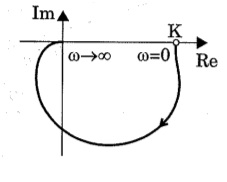
\includegraphics[angle = {-0.3}, width=3cm]{./images/PT2_Nyq.jpg}
	        \end{minipage}
			\begin{minipage}{9cm}
	        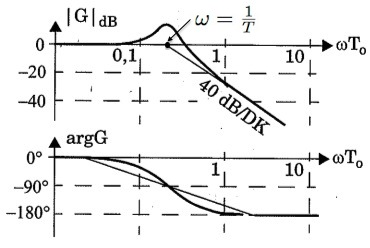
\includegraphics[angle = {0.2}, width=8cm]{./images/PT2_Bode.jpg}
	        \end{minipage} \rule[-5mm]{0mm}{35mm}
	        \\
			\specialrule{2pt}{0pt}{0pt}
			
			
			%Tt_Glied
			$T_t$ &
	        \parbox[c][2cm]{3cm}{\begin{tikzpicture}
  \begin{scope}[very thick]
    \draw[->] (0,0) -- +(0.5,0) node[near start, above] {u};
    \draw (0.5,-0.6) rectangle +(1.5,1.2);
    \draw[->] (2,0) -- +(0.5,0) node[near end, above] {y};
  \end{scope}

  \node at (0.7,0.9) {K};
  \node at (1.8,0.9) {D,$\omega_0$};

  % Inhalt
  \begin{scope}[shift={(0.8,-0.4)}]
    \draw[->, thick] (-0.2,0) -- +(1.3,0);
    \draw[->, thick] (0,-0.1) -- +(0,1);

    \draw[blue, very thick] (-0.2,0) -- ++(0.5,0) -- ++(0,0.7) -- +(0.6,0);
  \end{scope}

\end{tikzpicture}}
	        &
	        \begin{tabular}{lll}
	        	$y=\begin{cases}
  					0 & 0<t<T_t \\
  					u(t-T_t) & t \geq T_t
					\end{cases}$ & & \\
				$u=1(t)$ & $y=1(t-T_t)$ & \\
				$G(j \omega)= e^{-j\omega T_t}$ & $\left| G \right| = 1$ & $argG=-\omega T_t$
	        \end{tabular}
			\\ \cline{2-3}
			& \parbox[c][2cm]{3cm}{\begin{tikzpicture}
  \begin{scope}[very thick]
    \draw[->] (0,0) -- +(0.5,0) node[near start, above] {u};
    \draw (0.5,-0.6) rectangle +(1.5,1.2);
    \draw[->] (2,0) -- +(0.5,0) node[near end, above] {y};
  \end{scope}

% Zugemüse
\node at (1.8,0.9) {$T_t$};

\draw[very thick] (0.9,-0.6) -- ++(0,1) -- +(1.1,0);
\end{tikzpicture}}
			& 
			\parbox[c]{3cm}{\usetikzlibrary{decorations.markings}
\begin{tikzpicture}
\useasboundingbox (-1.4,-1.4) rectangle (1.9,1.4);
\draw[->, thick] (-1.1,0) -- (1.6,0) node[above] {Re};
\draw[->, thick] (0,-1) -- (0,1.1) node[left] {Im};

\draw (0.8,0.05) arc(90:450:0.05) node[above right] {\small{1}};
\draw (-0.8,0.05) arc(90:450:0.05) node[above left] {\small{-1}};

\draw[blue, thick,
	decoration={
		markings,
		mark= at position 0.9 with {\arrow{<}}
	},
	postaction={decorate}
] (0.8,0) arc (0:360:0.8);

\scalebox{0.7}{
  \node at (1.3,-1.5) {$2\pi$-periodisch};
  \node at (1.6, -0.3) {$\omega = 0$};
}
%\draw (current bounding box.south west) rectangle (current bounding box.north east);
\end{tikzpicture}}
			\parbox[c]{6cm}{\begin{tikzpicture}[xscale=1.5, yscale=0.8]
	%% Amplitude
\begin{scope}
	%% Koordinatensystem
	\draw[thick, ->] (0,-1.2) -- (0,0.5) node[right] {$|G|_{dB}$};
	\draw[dashed,gray] (1,-1.2) -- +(0,1.5);
	\draw[dashed,gray] (2,-1.2) -- +(0,1.5);
	\draw[dashed,gray] (3,-1.2) -- +(0,1.5);
	
	\draw[thick, ->] (-0.1,0.1) node[left] {$0$} -- +(3.6,0) node[right] {$\omega T_0$};
	\draw[dashed,gray] (0,-0.9) node[left, black] {$-40$} -- +(3.5,0);
	\draw[dashed,gray] (0,-0.4) node[left, black] {$-20$} -- +(3.5,0);

	%%%%%%%%%%%%%%%%

	%% Amplitudengang
	\draw[blue, very thick] (0,0.1) -- +(3.4,0);
\end{scope}


%% Phase
\begin{scope}[shift={(0,-2.2)}]
	%% Koordinatensystem
	\draw[thick, ->] (0,-1) -- (0,0.5) node[right] {$arg(G)$};
	\draw[dashed, gray] (1,-1) node[below, black] {$0.1$} -- +(0,1.2);
	\draw[dashed,gray] (2,-1) node[below, black] {$1$} -- +(0,1.2);
	\draw[dashed,gray] (3,-1) node[below, black] {$10$} -- +(0,1.2);
	
	\draw[thick, ->] (-0.1,0.2) node[left] {$0^\circ$} -- +(3.5,0) node[right] {$\omega T_0$};
	\draw[dashed,gray] (0,-0.3) node[left, black] {$-90^\circ$} -- +(3.5,0);
	\draw[dashed,gray] (0,-0.8) node[left, black] {$-180^\circ$} -- +(3.5,0);

	%%%%%%%%%%%%%%%%

	%% Amplitudengang
	\draw[blue, very thick] (0,0.2) .. controls (0.8,0.2) and (1.7,0.2) .. (2.3,-1.4);	
\end{scope}

%\draw (current bounding box.south west) rectangle (current bounding box.north east);
\end{tikzpicture}}
	        \\
			\specialrule{2pt}{0pt}{0pt}
		
		%DT1_Glied
			$DT_1$ &
	        \parbox[c][2cm]{3cm}{\begin{tikzpicture}
  \begin{scope}[very thick]
    \draw[->] (0,0) -- +(0.5,0) node[near start, above] {u};
    \draw (0.5,-0.6) rectangle +(1.5,1.2);
    \draw[->] (2,0) -- +(0.5,0) node[near end, above] {y};
  \end{scope}

 % Zugem�se
 \node at (0.7,0.9) {$T_V$};
 \node at (1.8,0.9) {$T_C$};
 \draw[very thick] (0.5,0.5)  .. controls (0.7,-0.1) and (1.4,-0.4) .. (2,-0.5);

\end{tikzpicture}}
	        &
	        \begin{tabular}{lll}
	        	$G(j \omega)= G_D \cdot G_{PT_1} = j\omega T_V \dfrac{1}{1+j\omega T_C} = \dfrac{T_V}{T_C}\left(1- \dfrac{1}{1+ j\omega T_C} \right)$ \\
	        \end{tabular}\\
	        \specialrule{2pt}{0pt}{0pt}
        \end{longtable}

%----------------------------------------------------------------------------------------
%
%	Tabelle aus Buch Seite 124
%
%
%	\subsection{Der Frequenzgang \formelbuch{117}}
%		\begin{tabular}{| c | c | c | c |}
%		    \hline
%	        $P$-Glied & $I$-Glied & $PT_1$-Glied & $T_t$-Glied \\
%	        \begin{minipage}{3cm}
%	        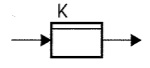
\includegraphics[width=3cm]{./images/pglied}
%	        \end{minipage} &
%			\begin{minipage}{3cm}
%	        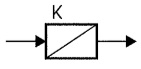
\includegraphics[width=3cm]{./images/iglied}
%	        \end{minipage} &
%			\begin{minipage}{4cm}
%	        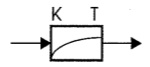
\includegraphics[width=3cm]{./images/pt1glied}
%	        \end{minipage} &
%			\begin{minipage}{3cm}
%	        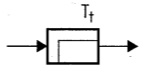
\includegraphics[width=3cm]{./images/tglied}
%	        \end{minipage} \\
%	        \hline
%	        $y=Ku$ & $\dot{y} = Ku$ & $T\dot{y}+y = Ku$ & $y=u(t-T_t)$ \\
%	        &  &  & $t\geq T_t$ \\
%	        \hline
%	        $G(j\omega)=K$ & $G(j\omega)= \frac{K}{j\omega}$ &
%	        $G(j\omega)=\frac{K}{1+j\omega T}$ &
%	        $G(j\omega)=e^{-j\omega T_t}$\\
%	        & & & \\
%	        \hline
%	        $\left| G \right| = K$ & $\left| G \right| = \frac{K}{\omega}$ &
%	        $\left| G \right| = \frac{K}{\sqrt{1+(|\omega T)^2}}$ &
%	        $\left| G \right| = 1$ \\
%	        $argG=0$ & $argG= -\frac{\pi}{2}$ & $argG=-\arctan(\omega T)$ &
%	        $argG= - \omega T_t$\\
%	        & & &  \\
%	        \hline
%	        & & & \\
%	        \begin{minipage}{3cm}
%	        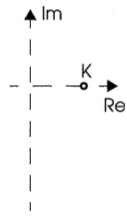
\includegraphics[width=2.7cm]{./images/fg_pglied}
%	        \end{minipage} &
%			\begin{minipage}{3cm}
%	        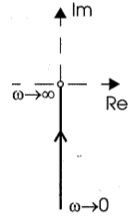
\includegraphics[width=3cm]{./images/fg_iglied}
%	        \end{minipage} &
%			\begin{minipage}{4cm}
%	        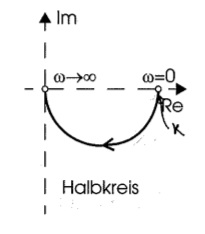
\includegraphics[width=4cm]{./images/fg_pt1glied}
%	        \end{minipage} &
%			\begin{minipage}{3cm}
%	        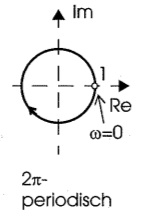
\includegraphics[width=3cm]{./images/fg_tglied}
%	        \end{minipage} \\
%			& & & \\
%	        \hline
%	        \end{tabular}

%----------------------------------------------------------------------------------------

	\newpage

	\subsection{Stabilitätsproblem \formelbuch{108}}
	\begin{multicols}{2}	
        
        \textbf{P-Glied mit Totzeit gegengekoppelt \formelbuch{109}}\\
        	$\bullet \; K_P < 1$: stabil\\
        	$\bullet \; K_P = 1$: grenzstabil\\
        	$\bullet \; K_P > 1$: instabil mit $\omega_{\pi} = \frac{2\pi}{T_t}$\\
        	$\omega_\pi$: Phasenschnittfrequenz
        	
       	\columnbreak
        	
		\textbf{I-Glied mit Totzeit gegengekoppelt \formelbuch{111}}\\
			Grenzkurve: \fbox{$K_I T_t=\frac{\pi}{2}$}, wobei \fbox{$\omega_\pi = K_I$}\\
        
        \textbf{Zwei I-Glieder gegengekoppelt \formelbuch{115}}\\
        	\fbox{$\omega_\pi = \sqrt{K}$}
	\end{multicols}
	Zur Instabilität führt das Zusammenwirken von Verstärkung und Signalverzögerung. Dabei ist die Reihenfolge der Glieder beliebig. Entscheiden sind gesamte Verstärkung $=$ Kreisverstärkung und gesamte Verzögerung $=$ Kreisverzögerung im offenen Regelkreis.

	\subsection{Nyquistkriterium \formelbuch{129}}
		\begin{minipage}{8cm}
			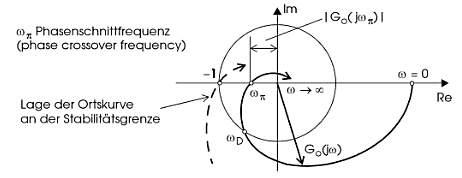
\includegraphics[width = 7.5cm]{./images/Nyquistkurve}
		\end{minipage}
		\begin{minipage}{10cm}
			Der geschlossene Regelkreis ist genau dann stabil, wenn beim Durchlauf der
			Ortskurve des offenen Regelkreise $G_o$ in Richtung zunehmender Frequenz der kritische Punkt -1 \glqq zur Linken\grqq\ liegt, daher nicht umschlungen wird. \\ \\ 
			Dies ist eine vereinfachte Form des Nyquist-Kriterium und setzt einen stabilen offenen Kreis voraus (Prozess mit Ausgleich), der auch noch durch ein I-Glied ergänzt sein darf (Prozess ohne Ausgleich).
		\end{minipage}
		 
		
	\subsection{Phasenreserve und Verstärkungsreserve \formelbuch{132}}
		\begin{tabular}{l|ll}
			$K_RK_{Rres}=K_{R\pi}$ & $K_R$ & Reglerverstärkung ($K_R < K_{R\pi} \rightarrow$ Regelung stabil, $K_R > K_{R\pi} \rightarrow$ Regelung
			instabil	) \\
			$K_{Rres}=\frac{1}{\left| G_o(j\omega_{\pi})\right|}$ & $K_{Rres}$ & 	Verstärkungsreserve mit Regler (Amplitudenres., gain margin) $\geq 4$ (praktisch) \\
			$K_{R\pi} = K_R \cdot \frac{1}{|G_o(j\omega_\pi)|}$ & $K_{R\pi}$ & kritische Verstärkung (Verstärkung ohne Regler) \\
			$argG_o(\omega_D)=-\pi+\Phi_{res}$ & $\omega_\pi$ & Phasenschnittfrequenz\\
			$|G_o(j\omega_D)|=1$ & $\omega_D$ & Durchtrittsfrequenz \\
			$argG_o(\omega_\pi)=-\pi$ & $\Phi_{res}$ & Phasenreserve (phase margin) $\Rightarrow 45^{\circ} \leq \Phi_{res} \leq 70^{\circ}$
		\end{tabular}
		\begin{minipage}{7cm}
			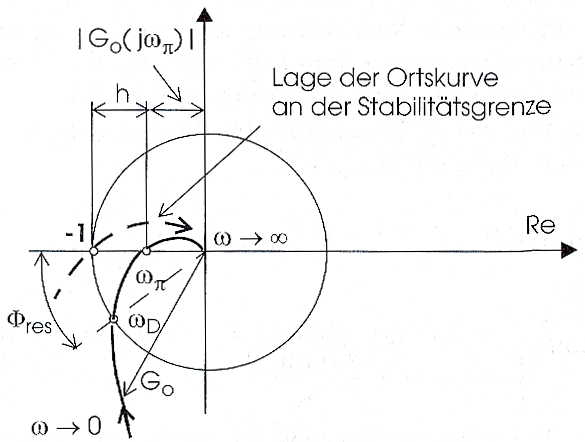
\includegraphics[width=6.5cm]{./images/phasenreserve.png}
		\end{minipage}
		\begin{minipage}{11cm}
			\subsubsection{Vorgehen beim Einstellen von P-Regler \formelbuch{133}}
			\textbf{Geg:} $\Phi_{res}$
			\begin{enumerate}
				\item Mit $argG_o(\omega_D) = -\pi + \Phi_{res} \rightarrow$ Durchtrittsfrequenz bestimmen.
				\item Mit $|G_o(j\omega_D)| = 1 \rightarrow$  Nach $K_{R}$ auflösen 
			\end{enumerate}
			\vspace{0.5cm}
			\textbf{Geg:} $K_{Rres}$
			\begin{itemize}
				\item $K_R = \dfrac{1}{K_{Rres} \cdot |G(j\omega_\pi)|}$, wobei bei $|G(j\omega_\pi)| \rightarrow K_R = 1$ gewählt.
			\end{itemize}
			
		\end{minipage}
        
			
	\subsection{Sprungantwort und Stabilität \formelbuch{135}}
		\subsubsection{Stabilitätssatz für ein geschlossenes System 2. Ordnung \formelbuch{137}}
			Ein System 2. Ordnung ist genau dann stabil, wenn {\bf alle} Koeffizienten der
			homogenen Dgl. positiv und ungleich 0 sind.\\
			$\ddot{y}+a_1\dot{y}+a_0y=F(u)$ \\
			Für $a_0 = 0$ und $a_1 > 0$ enthält der Prozess ein reines I-Glied und
			ist somit ein Prozess ohne Ausgleich.  \\ \\
			Bei LTI-Systemen höherer Ordnung genügt dieser Satz nicht. Er ist jedoch notwendig, daher müssen alle Koeffizienten vorhanden und positiv sein. Jedoch ist dies nicht hinreichend!
			
		\subsubsection{Stabilitätssatz für die Sprungantwort}
			Ein LTI-System ist genau dann stabil, wenn die Sprungantwort einem
			konstantem Wert zustrebt.

\newpage
\section{PID-Regler \formelbuch{147}}

	\subsection{P-Regler - Stationärer Zustand \formelbuch{155}}
		Beim einfachsten linearen Regler, dem P-Typ, besteht ein proportionaler
		Zusammenhang zwischen Fehler $e$ und Stellgrösse $u$.
		Der P-Regler reagiert schnell, kann aber den Sprungfehler nicht vollständig
		eliminieren. Er hat einen stationären Fehler. Eine zu hohe Verstärkung $K_R$ führt
    zu Rauschen.


	\subsection{I-Regler \formelbuch{160}}
		Der reine I-Regler ist allgemein ungünstig, weil er relativ langsam arbeitet
		und die Stabilität schwächt. Ist aber die Regelstrecke nur erster Ordnung
		erziehlt man gute Ergebnisse mit dem I-Regler.\\
		Der I-Regler neigt zum Schwingen.\\
		Bei sprungförmigen Signalen, d.h. für Festwertregelungen hat der I-Regler
		keinen Fehler!


	\subsection{PT$_2$-Glied \formelbuch{163}}
	\subsubsection{Parameter der Sprungantwort}
    \renewcommand{\arraystretch}{1.8}
    \begin{tabular}{|m{7cm}|m{1cm}m{0.5cm}m{8cm}}
      \cline{1-1}
      $y_{\infty} =A \cdot K$ & &
      $y_{\infty}$: & Endwert\\
      \cline{1-1}  
        $T_\omega = 2T_m=\dfrac{2\pi}{\omega_n \sqrt{1-\zeta^2}}=\dfrac{2\pi}{\omega}$ & &
        $T_{\omega}$: & Schwingungsdauer \\
      \cline{1-1}
      	$\varepsilon = \frac{\Delta y}{y_{\infty}}$ & &
      	$\varepsilon$: & Verhältnis von Überschwinger nach $T_e$ zum Endwert\\
      \cline{1-1}  
        $T_e = \dfrac{\ln\left(\varepsilon\sqrt{1-\zeta^2}\right)}{-\omega_n\cdot\zeta} = 
        \dfrac{1}{\sigma}\ln\left(\dfrac{\varepsilon\omega}{\omega_n}\right)$ & &
        $T_e$: & Einschwingzeit \\
      \cline{1-1}  
        $T_m = \dfrac{\pi}{\omega_n\sqrt{1-\zeta^2}}=\dfrac{\pi}{\omega}$ & &
        $T_m$: & Überschwingungsdauer\\
      \cline{1-1}  
      	$y_m = y_{\infty} \cdot e^{\frac{-\pi\cdot\zeta}{\sqrt{1-\zeta^2}}}$ & &
        $y_m$: & Überschwingweite\\
       \cline{1-1}  
        $\omega = \dfrac{1}{T}\sqrt{1-\zeta^2}= \omega_n\sqrt{1-\zeta^2}=\dfrac{2\pi}{T_\omega}=2\pi f$ & &
        $\omega$: & Kreisfrequenz \\
      \cline{1-1}  
        $\omega_n = \dfrac{1}{T}$ & &
        $\omega_n$: & Kennkreisfrequenz \\
      \cline{1-1}  
        $T_a = \frac{\pi - \arccos{(\zeta)}}{\omega_n\cdot\sqrt{1-\zeta^2}}$ & &
        $T_a$: & Anschwingzeit/Anregelzeit \\
      \cline{1-1}  
        $\sigma = -\dfrac{\zeta}{T} = -\zeta\omega_n$ & &
        $\zeta$: & Dämpfungskonstante \\
      \cline{1-1}  
        $\varepsilon =  \dfrac{\Delta y}{y_{\infty}}$ & &
        $\Delta y$: & Toleranzbereich der Amplitude im eingeschwungenen Zustand \\
      \cline{1-1}
      	$\delta = \ln{\Big(\frac{y_i}{y_{i+1}}\Big)} = \frac{2\pi \zeta}{\sqrt{1-\zeta^2}}$ & &
        $\delta$: & Logarithmisches Dekrement\\
      \cline{1-1}  
    \end{tabular}
    \renewcommand{\arraystretch}{1}
	
  \begin{multicols}{2}
	\subsubsection{Sprungantwort}
	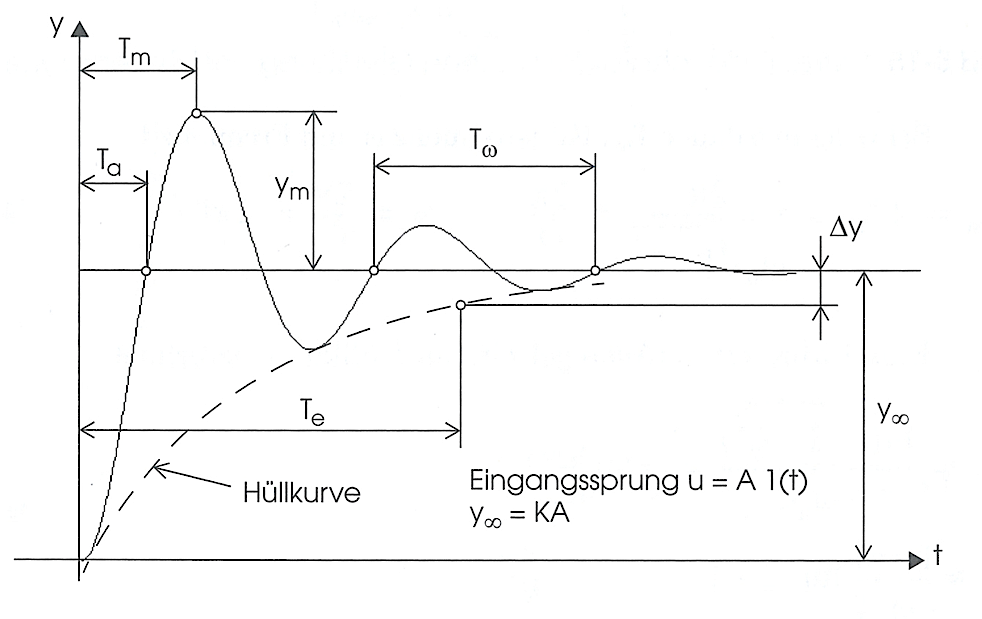
\includegraphics[width = 9cm]{./images/pt2StepResp}
	
	\subsubsection{Dämpfung}
	Optimal bei $\zeta=\frac{1}{\sqrt{2}}$ ($\Psi=45$).
	Dabei erreicht die Regelgrösse $y$ nach $4.3\%$ Überschwingen rasch den	Endwert.
		
    \subsubsection{Berechnung $\zeta$}
     \textbf{Aus DGL} $\ddot{y}+a_1\dot{y}+a_0 y=\ldots$ folgt $a_1=2\zeta\omega_n$, 
      $a_0=\omega_n^2$
      $\Rightarrow \zeta=\frac{a_1}{2\sqrt{a_0}}$ \\
      \textbf{Mittels Überschwingweite} kann $\zeta$ ebenfalls berechnet werden\\
      \begin{tabular}{p{2.5cm}p{2.5cm}p{4cm}}
        $\zeta = \frac{1}{\sqrt{1+(\frac{\pi}{c})^2}}$ & $c =ln(\frac{y_m}{y_{\infty}})$ & $y_m$: Überschwingweite
      \end{tabular}

		Weitere Formeln in der LTI-Grundglieder Tabelle
  \end{multicols}

	\subsection{PI-Regler \formelbuch{174}}
    \begin{tabular}{m{10cm}m{8cm}}
      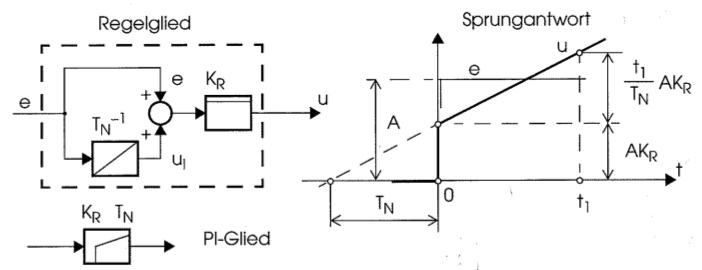
\includegraphics[width=10cm]{./images/PI_Regler.jpg} &
      {$u(t) = A \cdot K_R\left( 1 + \frac{t}{T_N}\right)$, wenn $e(t) = A \cdot 1(t)$ \newline
       \fbox{$G(j\omega)=K_R \dfrac{1+j\omega T_N}{j\omega T_N}$} \newline
       \fbox{$arg(G(j\omega))=\arctan(\omega T_N)-\dfrac{\pi}{2}$}\newline
       \fbox{$|G(j\omega)| = \dfrac{K_R \sqrt{1+(\omega T_n)^2}}{\omega T_n}$}
      \vfill
      }
    \end{tabular}


	\subsection{D-Glied  / $\text{DT}_1$-Glied \formelbuch{179/183}}
		Der Differenzierer erzeugt ein Korrektursignal im voraus.
		Nachteilig ist, wenn die Regelgrösse verrauscht ist, dann werden die
		hochfrequenten Störsignale durch die Ableitung verstärkt.\\
		Ein LTI-System, welches ohne D-Glied darstellbar ist, gegebenenfalls durch
		Umformung des Blockdiagramms, heisst realisierbar.  In der Realität wird
		meistens kein reines D-Glied sondern ein $DT_1$-Glied verwendet:\\ \\
    \begin{tabular}{|l||lll| l}
      \cline{1-4}
        \parbox[c][2cm]{3cm}{\begin{tikzpicture}
  \begin{scope}[very thick]
    \draw[->] (0,0) -- +(0.5,0) node[near start, above] {u};
    \draw (0.5,-0.6) rectangle +(1.5,1.2);
    \draw[->] (2,0) -- +(0.5,0) node[near end, above] {y};
    \draw(0.9, -0.2) rectangle +(1.1,0.8);
  \end{scope}

  \node at (0.7,0.9) {$K_D$};

\end{tikzpicture}} &
        \parbox[c][2cm]{4.5cm}{\begin{tikzpicture}
  %D-Glied
  \begin{scope}[very thick]
    \draw[->] (0,0) -- +(0.5,0) node[near start, above] {};
    \draw (0.5,-0.6) rectangle +(1.5,1.2);
    \draw[->] (2,0) -- +(0.5,0) node[near end, above] {};
    \draw(0.9, -0.2) rectangle +(1.1,0.8);
  \end{scope}

  \node at (0.7,0.9) {$T_V$};

  %PT1-Glied
  \begin{scope}[very thick]
    \draw (2.5,-0.6) rectangle +(1.5,1.2);
    \draw[->] (4,0) -- +(0.5,0) node[near end, above]{};
  \end{scope}

   % Zugem�se
   \node at (2.7,0.9) {1};
   \node at (3.8,0.9) {$T_C$};
   \draw[very thick] (2.5,-0.6)  .. controls (2.7,0.2) and (3.4,0.5) .. (4,0.5);

\end{tikzpicture}} &
        $\Rightarrow$ &
        \parbox[c][2cm]{3cm}{\begin{tikzpicture}
  \begin{scope}[very thick]
    \draw[->] (0,0) -- +(0.5,0) node[near start, above] {u};
    \draw (0.5,-0.6) rectangle +(1.5,1.2);
    \draw[->] (2,0) -- +(0.5,0) node[near end, above] {y};
  \end{scope}

 % Zugem�se
 \node at (0.7,0.9) {$T_V$};
 \node at (1.8,0.9) {$T_C$};
 \draw[very thick] (0.5,0.5)  .. controls (0.7,-0.1) and (1.4,-0.4) .. (2,-0.5);

\end{tikzpicture}} &
        \fbox{$G_{DT_1}(s) = \frac{j\omega T_V}{1+ j\omega T_C} = \frac{T_V}{T_C}\left(1- \frac{1}{1+j\omega T_C} \right) $}
        \\
        $D$-Glied &
        $D$-Glied \qquad $PT_1$-Glied & &
        $DT_1$-Glied \\
      \cline{1-4}
    \end{tabular}
    
    

	\subsection{PD-Regler \formelbuch{187/383}}
    \begin{tabular}{m{10cm}m{8cm}}
      {
        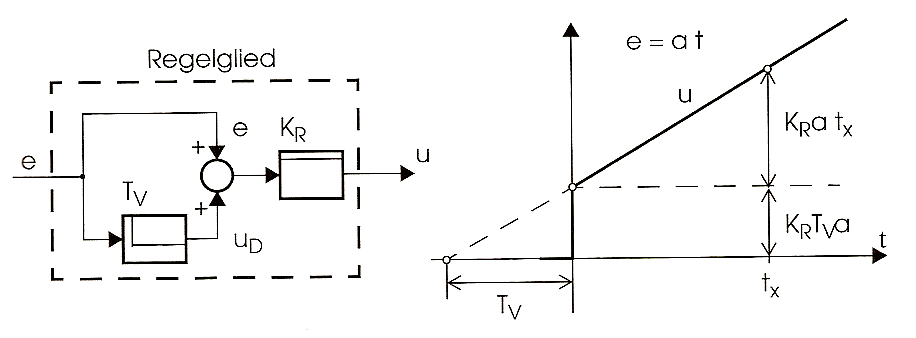
\includegraphics[width=10cm]{./images/PD_Regler.png}     \newline 
        Rampenantwort: $u(t) = K_R at+K_R T_V a$, wenn $ e(t) = a\cdot t$
      }&
      {
        Der PD-Regler entspricht dem inversen PT$_1$-Glied. Meistens wird jedoch
        der $PDT_1$ Regler verwendet.\newline
        Sprungantwort: \parbox{5cm}{$u(t) = K_R \left(1+\dfrac{T_V}{T_C}\cdot \e^{-\dfrac{t}{T_C}}\right)$, wenn $e(t) = 1(t)$} \newline
        \fbox{$G_{PDT_1}(j\omega) = K_R \dfrac{1+j\omega(T_V+T_C)}{1+j\omega T_C}$} \quad $T_V > T_C$
      }
    \end{tabular}
 

	\subsection{PID-Regler \formelbuch{183/383}}
    \begin{tabular}{m{9cm}|m{10cm}}
      \textbf{additive Form}(Parallelschaltung) & multiplikative Form (Serienschaltung) \\
      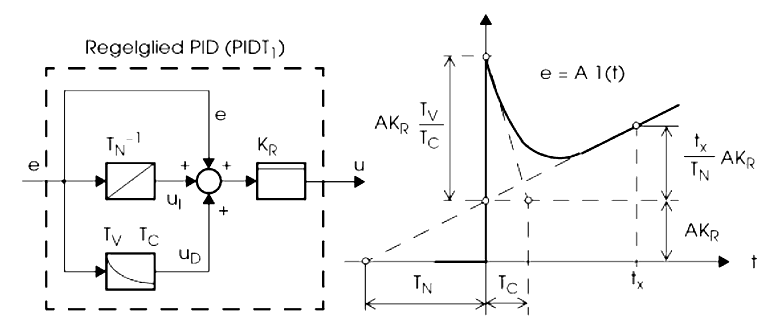
\includegraphics[width=9cm]{./images/PID_Regler_add} &
      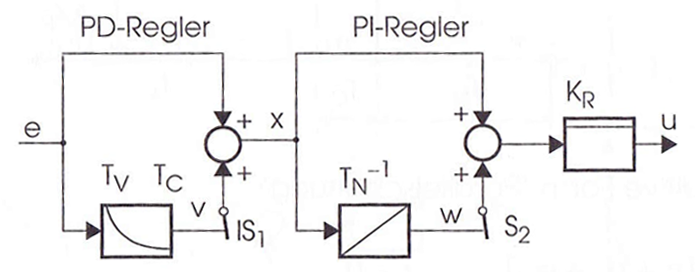
\includegraphics[width = 7cm]{./images/PID_Regler_mul}
      \\
      {
        \fbox{$G_{PIDT_1}(s) = K_R \left(1 + \frac{1}{s T_N} + \frac{s T_V}{1+s T_C} \right)$} \newline
        $e(t) = 1(t) \rightarrow u(t) = K_R \left( 1 + \frac{t}{T_N} + \frac{T_V}{T_C}e^{-\frac{t}{T_C}}\right)$
      } & 
      {
        \fbox{$G_{PIDT_1}(s) = K_R \frac{1+sT_N}{s T_N} \frac{1 + s(T_V + T_C)}{1+s T_C}$} \newline
        $e(t) = 1(t) \rightarrow u(t) = K_R \left[ 1 + \frac{T_V}{T_N} +\frac{t}{T_N} + \left( \frac{T_V}{T_C}-\frac{T_V}{T_B}\right)e^{-\frac{t}{T_C}}\right]$
      }
      \\
      \multicolumn{2}{c}{Praktisch ist: $T_N \leq T_V > T_C$}
      \\
    \end{tabular}
		

	\subsection{Empirische Einstellregeln \formelbuch{188}}
		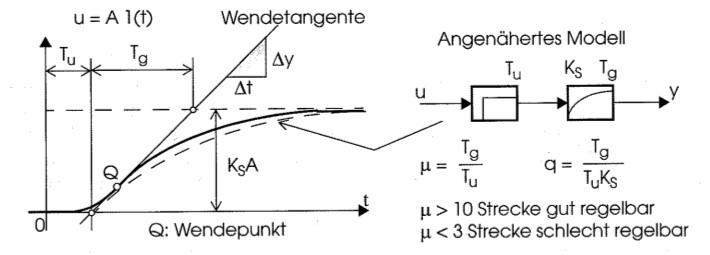
\includegraphics[width=13cm]{./images/Empirisch_Regeln.jpg}
		\begin{minipage}[b]{5cm}
        UTF des angenäherten Modells:\\ \\
		$G_0(j\omega)=\frac{K_s}{1+j\omega T_g}e^{-j\omega T_u}$
		\vspace{2.7cm}
		\end{minipage}\\

	\begin{tabular}{|l|p{1.8cm}|l|l|l|l||l|l|}
	    \hline
	    \multicolumn{6}{|c||}{
	      \textbf{Reglereinstellung nach Chien-Hrones-Reswick}
	    } &
	    \multicolumn{2}{|c|}{
	      \textbf{Reglereinstellung nach Ziegler-Nichols}
	    }
		\\ \hline
		\multicolumn{6}{|c||}{
		  $
		  q = \frac{T_g}{T_uK_S} \qquad \mu = \frac{T_g}{T_u}
		  \qquad \text{wenn} \quad \mu
		  \begin{cases}
		    > 10 \rightarrow \text{Strecke gut regelbar} \\
		    < 3 \rightarrow \text{Strecke schlecht regelbar}
		  \end{cases}
		  $
		} & $q=\frac{T_g}{T_uK_s}$ & $K_{R\pi} \qquad T_\pi=\frac{2\pi}{\omega_\pi}$
		\\ \hline
		\textbf{Regler} & \textbf{Regler\-parameter} &
		\multicolumn{2}{|p{3.5cm}|}{\textbf{Führungsverhalten} \newline $y_m$:
		Überschwingen} &
		\multicolumn{2}{|c||}{\textbf{Störverhalten}} &
		\textbf{Sprungantwort} & \textbf{Stabilitätsgrenze}
		\\ \hline
		& & kein $y_m$ & $\frac{y_m}{y_\infty} = 20 \%$ & kein $a$ & $\frac{a}{b}= 20 \%$ & &
		\\ \hline
		P 	& $K_R$ 	& $0.3q$ 	& $0.7q$ 	& $0.3q$ 	& $0.7q$	& $q$ 	& $0.5K_{R\pi}$
		\\ \hline
		PI	& $K_R$		& $0.35q$	& $0.6q$	& $0.6q$	& $0.7q$	& $0.9q$ 	& $0.45K_{R\pi}$
		\\
		    & $T_N$		& $1.17T_g$	& $1T_g$	& $4T_u$	& $2.33T_u$ & $3.33T_u$ &
		    $0.85T_{\pi}$ \\ \hline
		PID & $K_R$		& $0.6q$	& $0.95q$	& $0.95q$	& $1.2q$ 	& $1.2q$ 	& $0.60K_{R\pi}$
		\\
			& $T_N$		& $1T_g$	& $1.36T_g$	& $2.38T_u$	& $2T_u$ 	& $2T_u$	& $0.50T_\pi$
		\\
			& $T_V$		& $0.5T_u$	& $0.47T_u$	& $0.42T_u$	& $0.42T_u$ & $0.5T_u$ 	& $0.125T_\pi$
		\\ \hline
	\end{tabular}
  
  Empirisch Einstellregeln ergeben praktisch nicht immer das bestmögliche Zeitverhalten,
  sondern sie liefern eine erste Einstellung, welche experimentell noch verbessert werden kann.


	\subsection{Wind-Up \formelbuch{200}}
  \begin{tabular}{lp{15cm}}
    \textbf{Definition:} &
    Der Fehler $e$ am Integratoreingang bleibt konstant, sodass dessen
    Ausgangssignal ständig zunimmt. \\
    
    \textbf{Folge:} & 
    Einerseits ein konstanter Fehler und andererseits eine verzögert reagierende
    und damit stark überschwingende Regelgrösse $y$.
  \end{tabular}

  \begin{multicols}{2}
    \textbf{Ursachen für Wind-Up:}
    \begin{itemize}[leftmargin=*]
      \item I-Anteil
      \item Sättigung am Regler Ausgang
      \item $e(t)$ über "`längere Zeit"' $\neq 0$ ist.
    \end{itemize}
  
  \columnbreak
    
    \textbf{Anti-Wind-Up:}
    \begin{itemize}[leftmargin=*]
      \item Integration beschränken
    \end{itemize}
  
  
  \end{multicols}
  
  


\section{Diverses}
	\subsection{Frequenzgang zweier Systeme mit Rückkopplung }
		\begin{center}
    		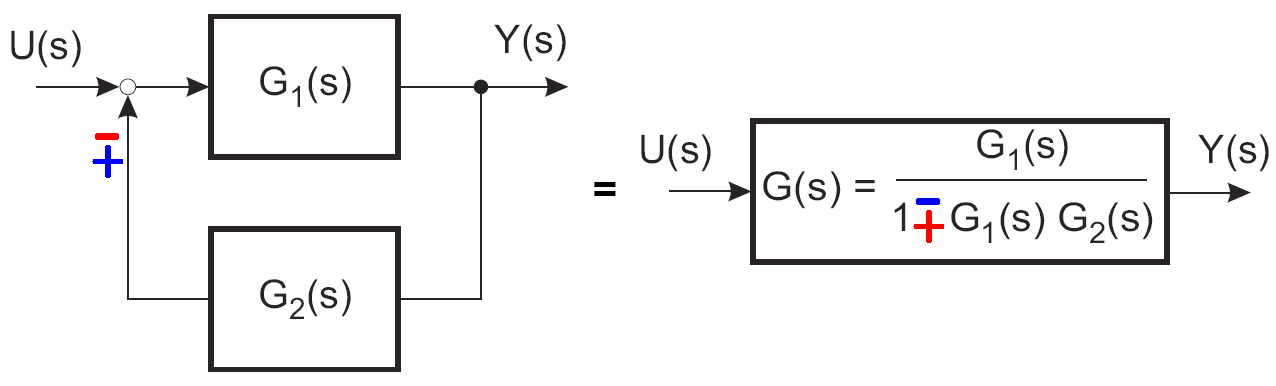
\includegraphics[height=3cm]{./bilder/feedback.png} \\
    		$G(s) = \frac{Y(s)}{U(s)}$
        \end{center}
    
    \subsection{Von $G(s)$ zur DGL}
    	\begin{multicols}{2}
    		\begin{itemize}
  				\item $G(s)$ als Bruch aufschreiben.
  				\item Zähler = Eingang ($u$) \quad Nenner = Ausgang ($y$)
  				\item $j\omega = \dot{y} \quad (j\omega)^2 = \ddot{y} \quad \ldots $
  				\item Gleiches gillt für den Zähler mit u!
			\end{itemize}
			\columnbreak
			\textbf{Beispiel:} $G(s) = \frac{K(j \omega T + 1)}{(j\omega)^2 T_N + j \omega Tn(1+K_R) + K_R}$ \\			
			\textbf{DGL:} $T_N \ddot{y} + T_N(1+K_R) \dot{y} + K_R y = K(T \dot{u} + u)$
    	\end{multicols}    	
    
    \subsection{Zeigerdiagramme}
    Soll zu einem Gegebenen Blockschaldbild (oder einer gegebenen Funktion) das Zeigerdiagramm erstellt 
    werden werden die \textbf{Beträge} der Elemente \textbf{multipliziert},
    die \textbf{Winkel} ($arg()$) \textbf{addiert}. Die Werte für die einzelnen Elemente sind der Tabelle in 1. LTI-Grundglieder zu entnehmen. 


	\subsection{Graphisch Phasen-/Verstärkungsreserve}
		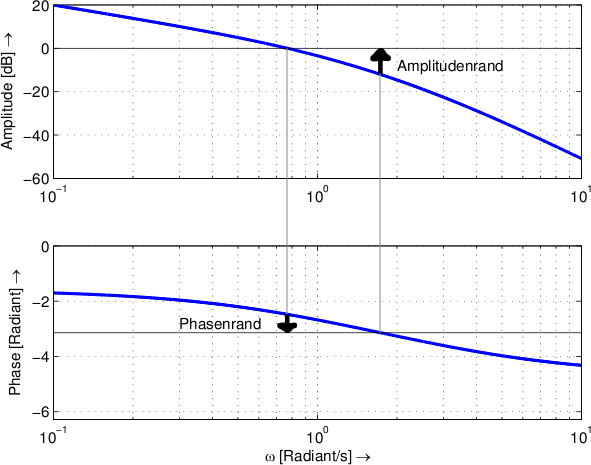
\includegraphics[width=7cm]{./bilder/bode-stabilitaet.png} \\
		Phasen-/Verstärkungsreserve = Phasen-/Amplitudenrand
		
\section{Umformungen}
 \begin{multicols}{2}
	\subsection{Serielle Systeme}
		\begin{tikzpicture}
  \node (G1) at (1,0) [draw]{$G_1(s)$};

  \node (G2) at (3,0) [draw]{$G_2(s)$};

  \draw [->] (0,0) --  (node cs:name=G1) --  (node cs:name=G2)  -- ++(1,0);
\end{tikzpicture}


		$G(s) = G_1(s) \cdot G_2(s)$
	\subsection{Parallele Systeme}
		\begin{tikzpicture}
  \node (in) at (0,1) []{u};
  \node (dot) at (1,1) [draw,circle,inner sep=1,fill]{};

  \node (G1) at (3,2) [draw]{$G_1(s)$};
  \node (G2) at (3,0) [draw]{$G_2(s)$};

  \node (sum) at (5,1) [circle,draw]{+};
  \node (out) at (6,1) []{y};


  \draw (in) -> (dot);
 
  \draw[->] (dot) |-  (G1);
  \draw[->] (G1) -| (sum);

  \draw[->] (dot) |-  (G2);
  \draw[->] (G2) -| (sum);

  \draw[->](sum) -- (out);

\end{tikzpicture}


		$G(s) = G_1(s) + G_2(s)$
	\subsection{Zwei Systeme mit Rückkopplung}
		\begin{tikzpicture}
  \node (in) at (0,2) []{$U(s)$};
  \node (sum) at (1,2) [circle,draw,inner sep=2]{};
  \node (G1) at (2.5,2) [draw]{$G_1(s)$};
  \node (G2) at (2.5,1) [draw]{$G_2(s)$};
  \node (dot) at (4,2) [draw,circle,inner sep=1,fill]{};
  \node (out) at (5,2) []{$Y(s)$};

  \node (feedback) at (sum) [below left] {$\pm$};

  \draw[->] (in) -- (sum);
  \draw[->] (sum) --  (G1);
  \draw (G1) --  (dot);
  \draw[->](dot) -- (out);

  \draw[->] (dot) |-(G2);
  \draw[->] (G2) -| (sum);

\end{tikzpicture}

\newline
		$G(s) = \frac{G_1(s)}{1 \mp G_1(s) G_2(s)}$ Vorzeichenwechsel! \\
		
		\begin{tikzpicture}
  \node (in) at (0,2) []{$U(s)$};
  \node (sum) at (1,2) [circle,draw,inner sep=2]{};
  \node (G1) at (5,2) [draw]{$G_1(s)$};
  \node (G2) at (2.5,1) [draw]{$G_2(s)$};
  \node (dot) at (4,2) [draw,circle,inner sep=1,fill]{};
  \node (out) at (6.5,2) []{$Y(s)$};

  \node (feedback) at (sum) [below left] {$\pm$};

  \draw[->] (in) -- (sum);
  \draw (sum) --  (dot);
  \draw[->] (dot) --  (G1);
  \draw[->](G1) -- (out);

  \draw[->] (dot) |-(G2);
  \draw[->] (G2) -| (sum);

\end{tikzpicture}
\newline
		$G(s) = G_1(s) \cdot \frac{1}{1 \mp G_2(s)}$ Vorzeichenwechsel!
		
  \end{multicols}
	\subsection{Komplexeres Beispiel}
		\begin{tikzpicture}
  \node (in) at (0,2) []{u};
  \node (G1) at (1.5,2) [draw]{$G_1(s)$};

  \node (sum) at (3,2) [circle,draw,inner sep=1]{+};

  \node (G2) at (4.5,2) [draw]{$G_2(s)$};
  \node (G3) at (4.5,1) [draw]{$G_3(s)$};

  \node (dot) at (6,2) [draw,circle,inner sep=1,fill]{};
  \node (G4) at (7.5,2) [draw]{$G_4(s)$};
  \node (out) at (9,2) []{y};


  \draw[->] (in) -- (G1);
 
  \draw[->] (G1) --  (sum);
  \draw[->] (sum) --  (G2);

  \draw (G2) -- (dot);
  \draw[->] (dot) |-(G3);
  \draw[->] (G3) -| (sum);

  \draw[->] (dot) |-  (G4);
  \draw[->](G4) -- (out);

\end{tikzpicture}


		$G(s) = G_1(s) \cdot \frac{G_2(s)}{1-G_2(s) \cdot G_3(s)} \cdot G_4(s)$


\end{document}
